\documentclass[bookmarks=true,bookmarksopen=true,pdfborder={0 0 0},pdfhighlight={/N},linkbordercolor={.5 .5 .5},implicit=false,unicode,xcolor={table}]{beamer}

\usepackage{cmsrb}
\usepackage[T1]{fontenc}
\usepackage[main=serbian, english]{babel}
\usepackage[utf8]{inputenc} 

\mode<presentation>
\setbeamercovered{transparent}
\setbeamertemplate{navigation symbols}{}

\usetheme{Frankfurt}
\usecolortheme{default}

\usepackage{color}
%\usepackage[table]{xcolor}
\usepackage{url}

\usepackage{graphicx}
\usepackage{xspace}
\usepackage{fancyvrb}
\usepackage{listings}
\usepackage{amsmath}
\usepackage{float}
\usepackage{xcolor}
\usepackage[normalem]{ulem}
\usepackage{subcaption}


\graphicspath{ {../thesis/images/} }
\usepackage{subcaption}
\captionsetup{compatibility=false}

\definecolor{mygreen}{rgb}{0,0.6,0}
\definecolor{mygray}{rgb}{0.5,0.5,0.5}
\definecolor{mymauve}{rgb}{0.58,0,0.82}

\lstset{ 
  backgroundcolor=\color{white},   % choose the background color; you must add \usepackage{color} or \usepackage{xcolor}; should come as last argument
  basicstyle=\scriptsize\ttfamily,        % the size of the fonts that are used for the code
  breakatwhitespace=false,         % sets if automatic breaks should only happen at whitespace
  breaklines=true,                 % sets automatic line breaking
  captionpos=b,                    % sets the caption-position to bottom
  commentstyle=\color{mygreen},    % comment style
  deletekeywords={...},            % if you want to delete keywords from the given language
  escapeinside={\%*}{*)},          % if you want to add LaTeX within your code
  extendedchars=true,              % lets you use non-ASCII characters; for 8-bits encodings only, does not work with UTF-8
  firstnumber=1,                % start line enumeration with line 1000
  frame=single,	                   % adds a frame around the code
  keepspaces=true,                 % keeps spaces in text, useful for keeping indentation of code (possibly needs columns=flexible)
  keywordstyle=\color{blue},       % keyword style
  language=C,                      % the language of the code
  morekeywords={*,...},            % if you want to add more keywords to the set
  numbers=left,                    % where to put the line-numbers; possible values are (none, left, right)
  numbersep=5pt,                   % how far the line-numbers are from the code
  numberstyle=\tiny\color{mygray}, % the style that is used for the line-numbers
  rulecolor=\color{black},         % if not set, the frame-color may be changed on line-breaks within not-black text (e.g. comments (green here))
  showspaces=false,                % show spaces everywhere adding particular underscores; it overrides 'showstringspaces'
  showstringspaces=false,          % underline spaces within strings only
  showtabs=false,                  % show tabs within strings adding particular underscores
  stepnumber=1,                    % the step between two line-numbers. If it's 1, each line will be numbered
  stringstyle=\color{mymauve},       % string literal style
  tabsize=2,	                   % sets default tabsize to 2 spaces
  title=\lstname                   % show the filename of files included with \lstinputlisting; also try caption instead of title
}

\setbeamertemplate{itemize item}[circle]
\setbeamertemplate{itemize subitem}[square]

\AtBeginSection[]{
  \begin{frame}
  \vfill
  \centering
  \begin{beamercolorbox}[sep=8pt,center,shadow=true,rounded=true]{title}
    \usebeamerfont{title}\insertsectionhead\par%
  \end{beamercolorbox}
  \vfill
  \end{frame}
}

\foreignlanguage{serbian}

\begin{document}

\title{Predviđanje trajektorija više objekata na sceni}
\author{Momir Adžemović}
\subtitle{}
\institute{Matematički fakultet \\ Univerzitet u Beogradu}
\date{23. septembar 2022.}

\begin{frame}

  \titlepage{}

\end{frame} 

\begin{frame}{Autonomna vožnja}

  \begin{itemize}
    \item Potpuna ili parcijalna automatizacija kontrole vozila
    \item Nivo 0: Čovek ima potpunu kontrolu nad vozilom
    \item ...
    \item Nivo 5: Računar (agent) ima potpunu kontrolu nad vozilom u svakom trenutku
  \end{itemize}

\end{frame}

\begin{frame}{Problem}

  \begin{itemize}
    \item Kratkoročna estimacija kretanja agenta nekoliko trenutaka u budućnosti (3 sekunde)
    \item Informacije:
      \begin{itemize}
        \item Istorija kretanja agenta
        \item Dinamički deo scene: Istorija kretanja objekata u okolini --- drugi vozači i pešaci
        \item Statičko okruženje agenta (put, pešački prelaz, semafori, itd.)
      \end{itemize}
  \end{itemize}

\end{frame}

\begin{frame}{Izazovi}

  \begin{itemize}
    \item Obrada i razumevanje podataka sa scene
    \item Stohastička priroda vozača --- Multimodalna raspodela krajnjih tačaka trajektorija (postojanje više izraženih lokalnih maksimuma)
  \end{itemize}

  \begin{figure}
		\begin{subfigure}{5.5cm}
			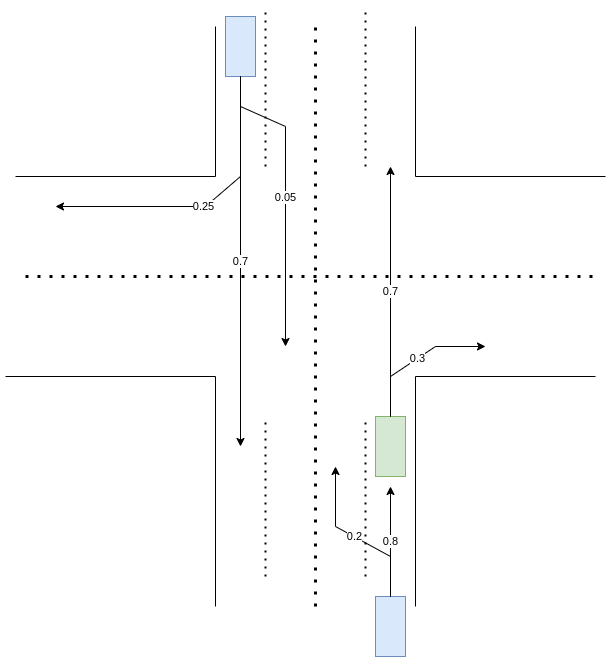
\includegraphics[width=5.5cm,height=5.5cm]{multimodal.drawio.png}
		\end{subfigure}
	\end{figure}
  \hfill
  
\end{frame}

\begin{frame}{Mape sa visokim nivoom detalja}

  \begin{itemize}
    \item Sadrži informacije o elementima scene i njihovim lokacijama sa greškom do par centimetara
    \item Superiorne u odnosu na GPS
    \item Za prikupljanje podataka se koriste \textit{LiDAR} sistemi
  \end{itemize}

  \begin{figure}
		\begin{subfigure}{5cm}
			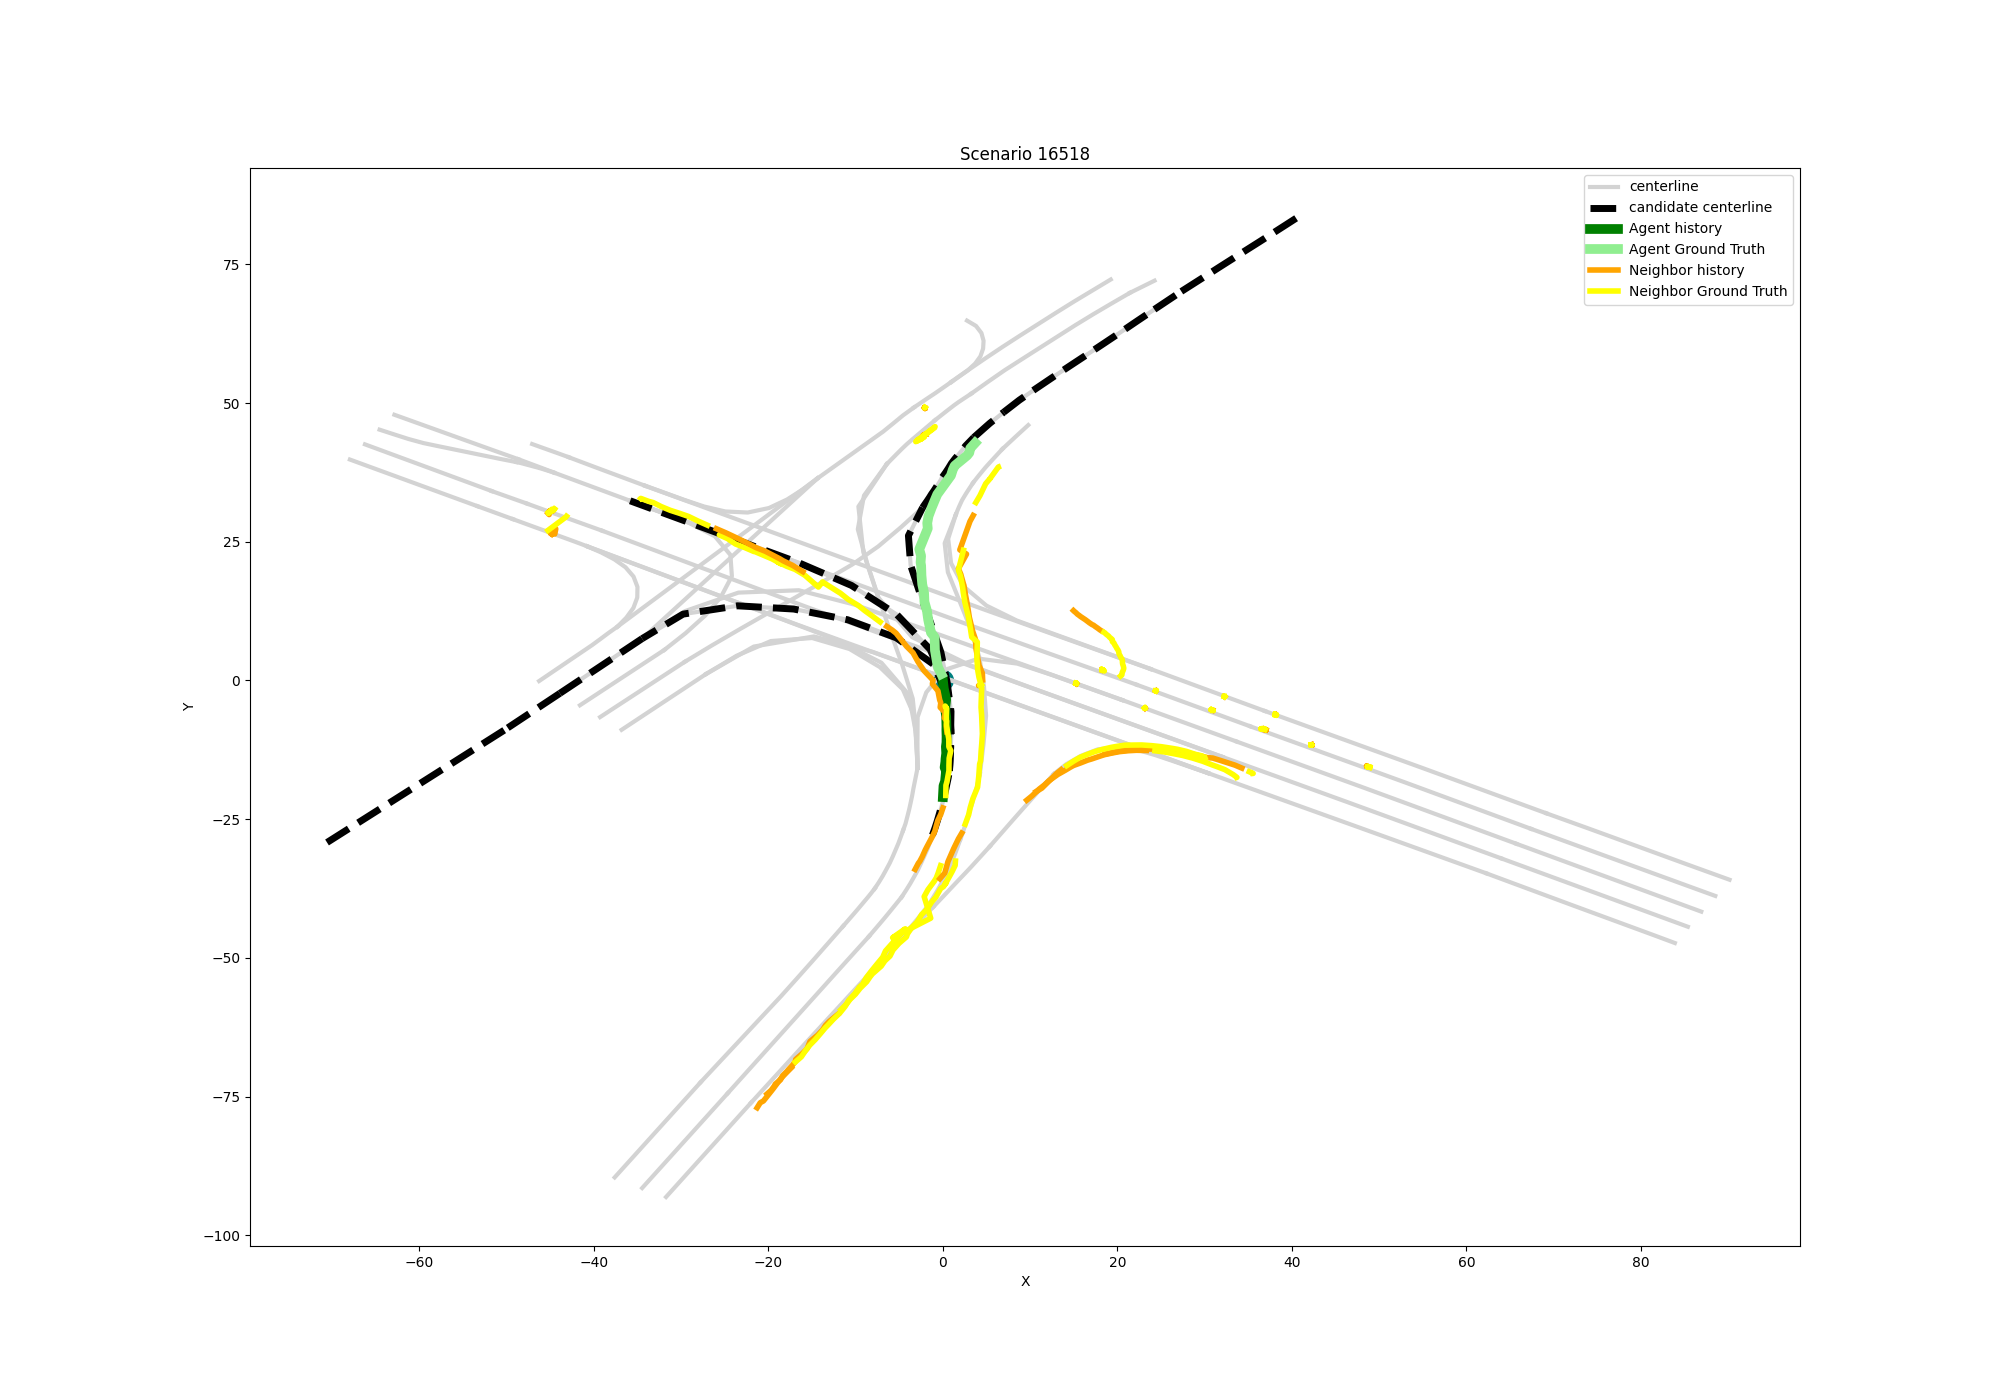
\includegraphics[width=5cm,height=4cm]{scenario_MIA_16518.png}
		\end{subfigure}
    \begin{subfigure}{5cm}
			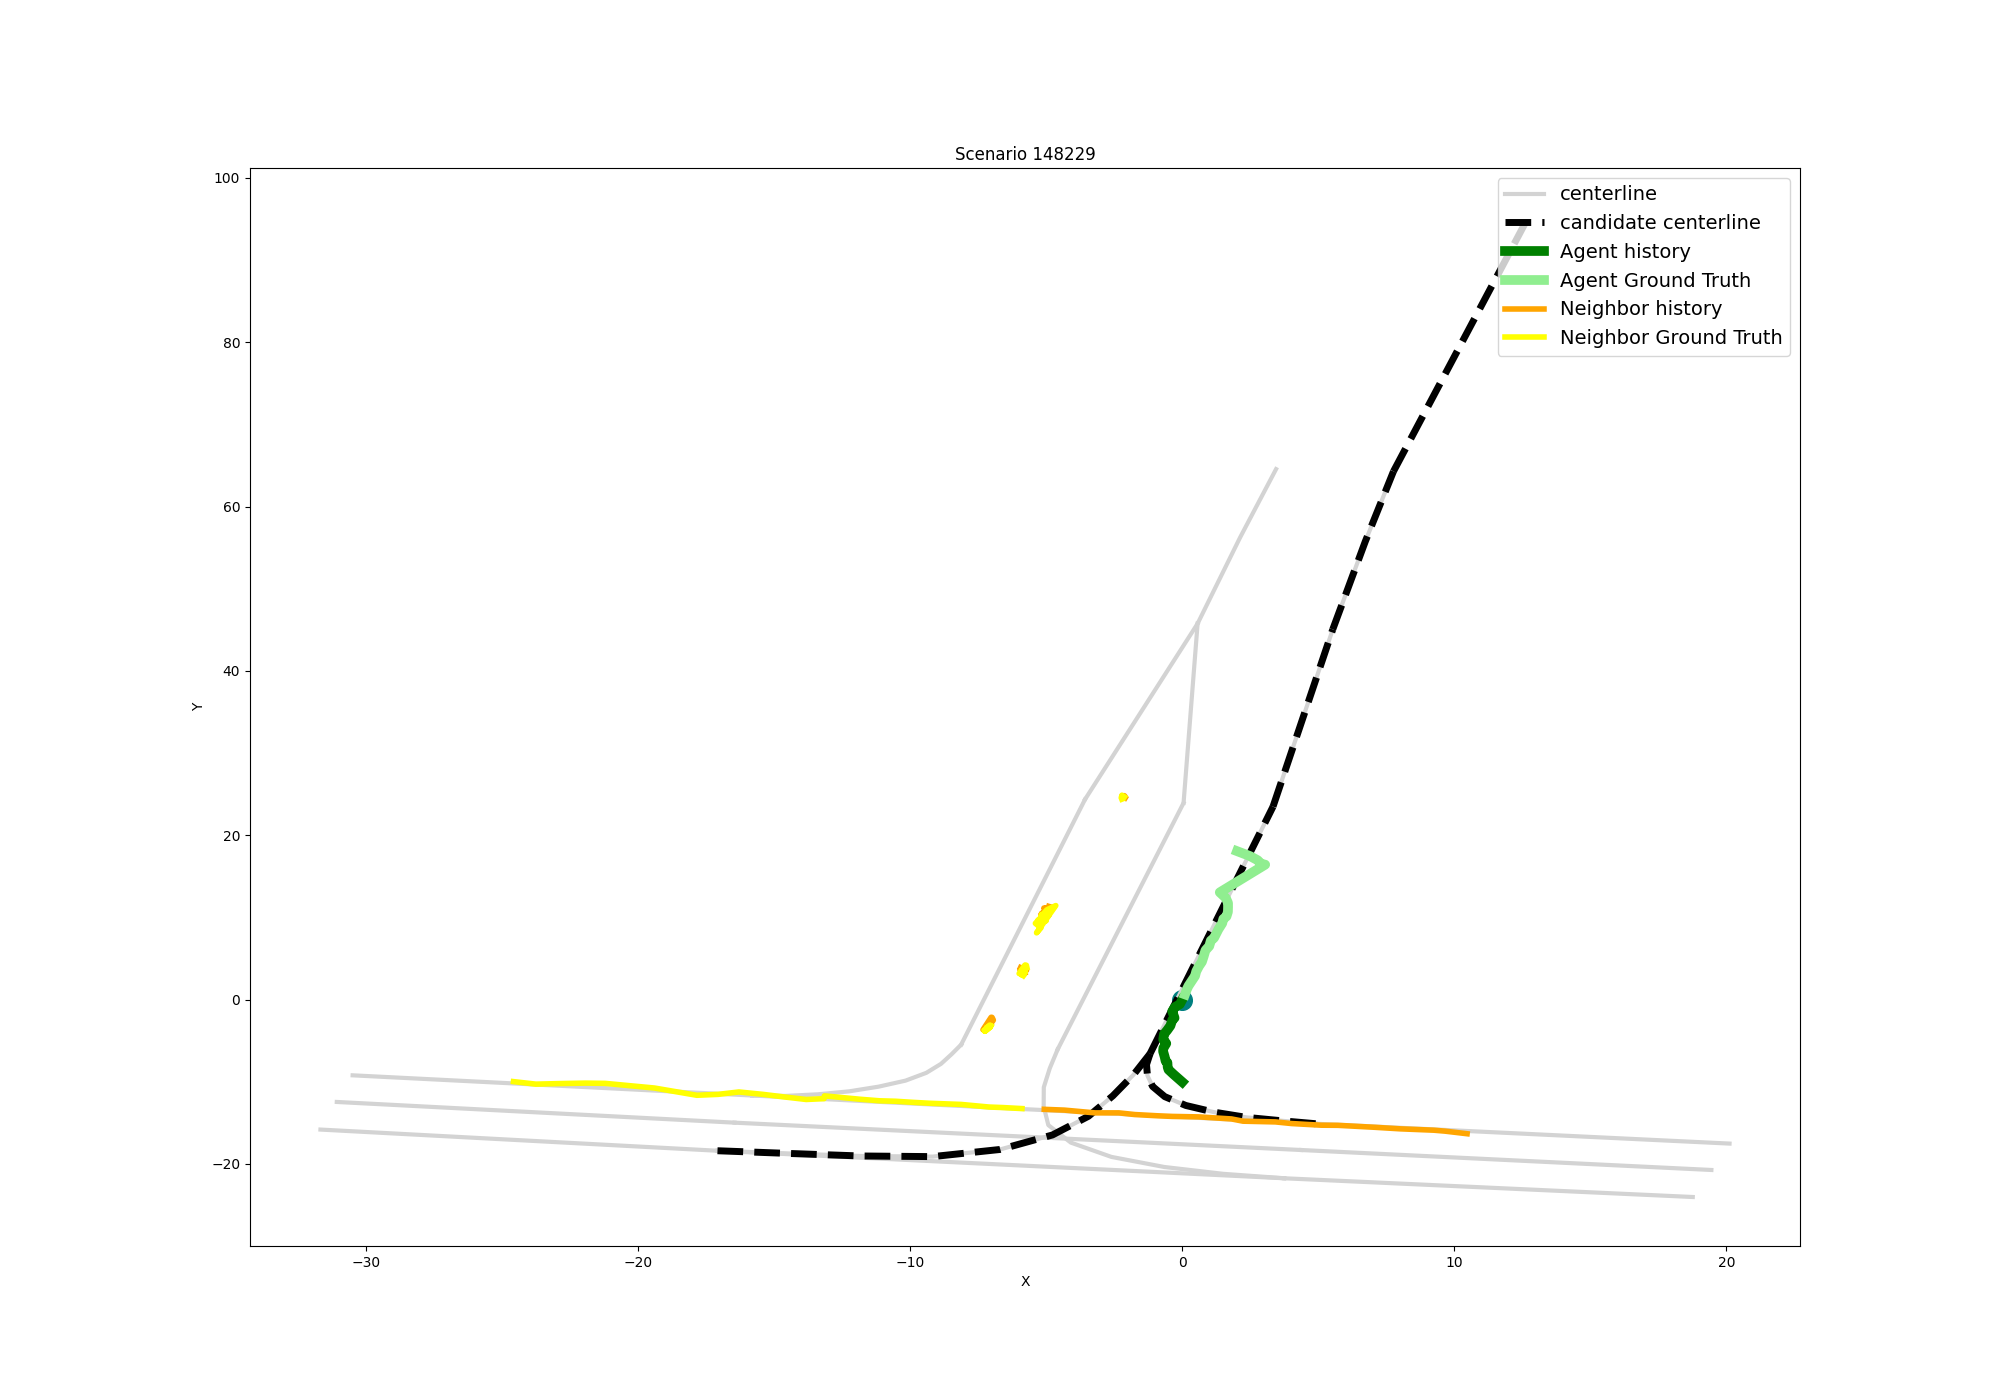
\includegraphics[width=5cm,height=4cm]{scenario_MIA_148229.png}
		\end{subfigure}
	\end{figure}

\end{frame}

\begin{frame}{VectorNet}
  
  \begin{itemize}
    \item Hijerarhijska grafovska neuronska mreža
    \item Komponente:
      \begin{itemize}
        \item Podgraf
        \item Globalni graf interakcija
        \item Predviđanje trajektorija
      \end{itemize}
  \end{itemize}


  \begin{figure}
    \begin{subfigure}{9cm}
      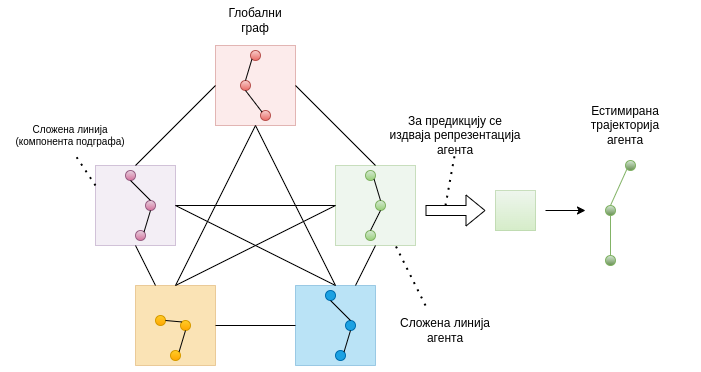
\includegraphics[width=9cm,height=5cm]{vectornet-overview-Hijearhija.drawio.png}
    \end{subfigure}
  \end{figure}
  \hfill

\end{frame}

\begin{frame}{TNT-VectorNet}

  \begin{itemize}
    \item Bolje performanse
    \item Uzorkovanje krajnjih tačaka trajektorija na osnovu heuristike
    \item Estimacija više od jedne trajektorije na osnovu uzorkovanih krajnjih tačaka
  \end{itemize}

  \begin{figure}
		\begin{subfigure}{5cm}
			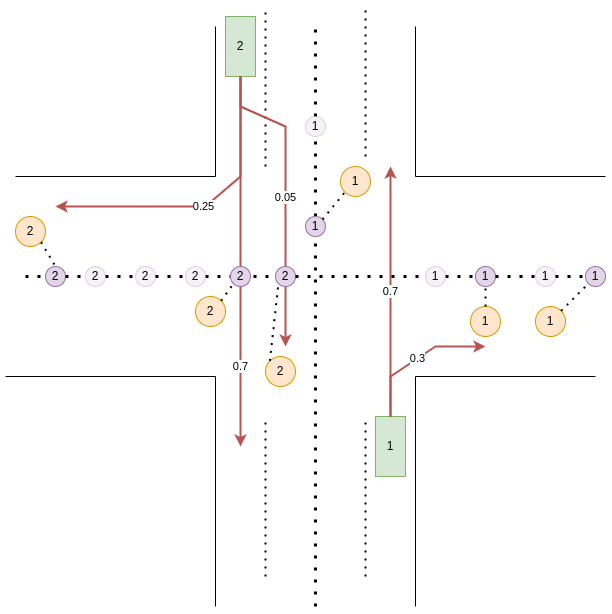
\includegraphics[width=5cm,height=5cm]{tnt-viz-Page-1.drawio.png}
		\end{subfigure}
    \hfill
    \begin{subfigure}{5cm}
			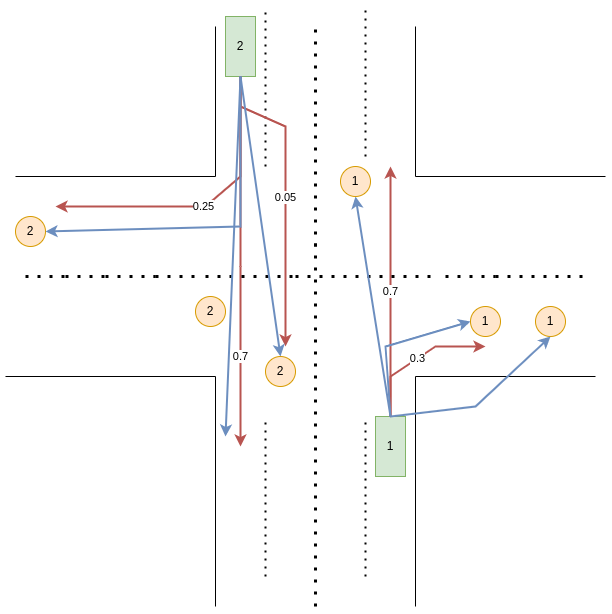
\includegraphics[width=5cm,height=5cm]{tnt-viz-Page-2.drawio.png}
		\end{subfigure}
	\end{figure}
  
\end{frame}

\begin{frame}{TNT-VectorNet: Rezultati}
  \centerline{$minADE_{6}$: $1.03$, $minFDE_{6}$: $1.91$, $MissRate^{2m}_{6}$: $0.30$}

  \begin{figure}
		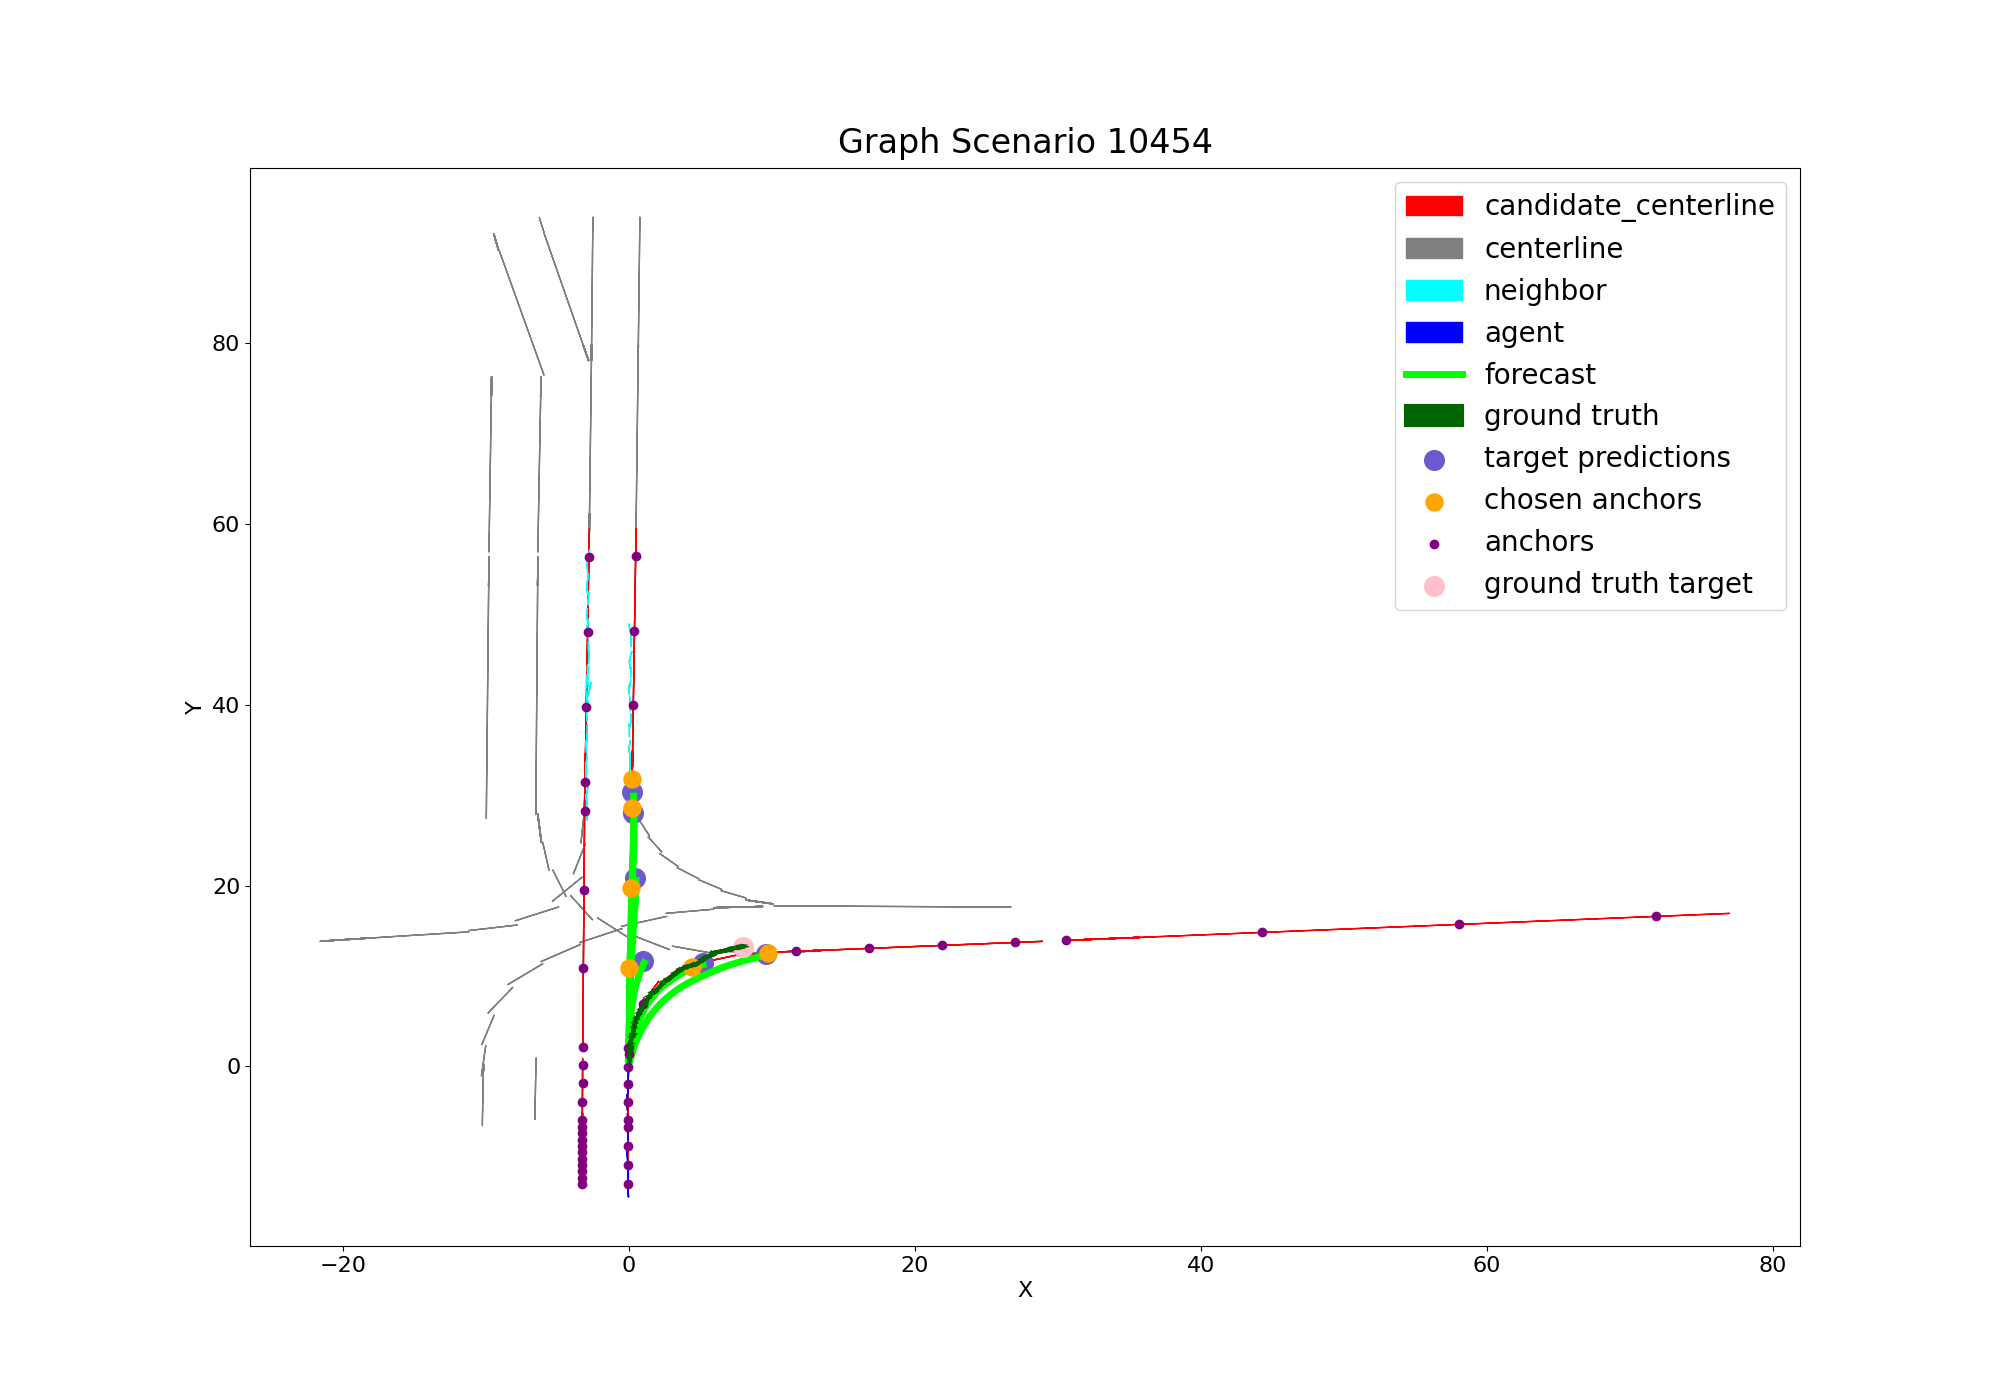
\includegraphics[width=9cm,height=6cm]{result_MIA_10454.png}
	\end{figure}
  
\end{frame}

\begin{frame}{TNT-VectorNet: Rezultati}
  \begin{figure}
		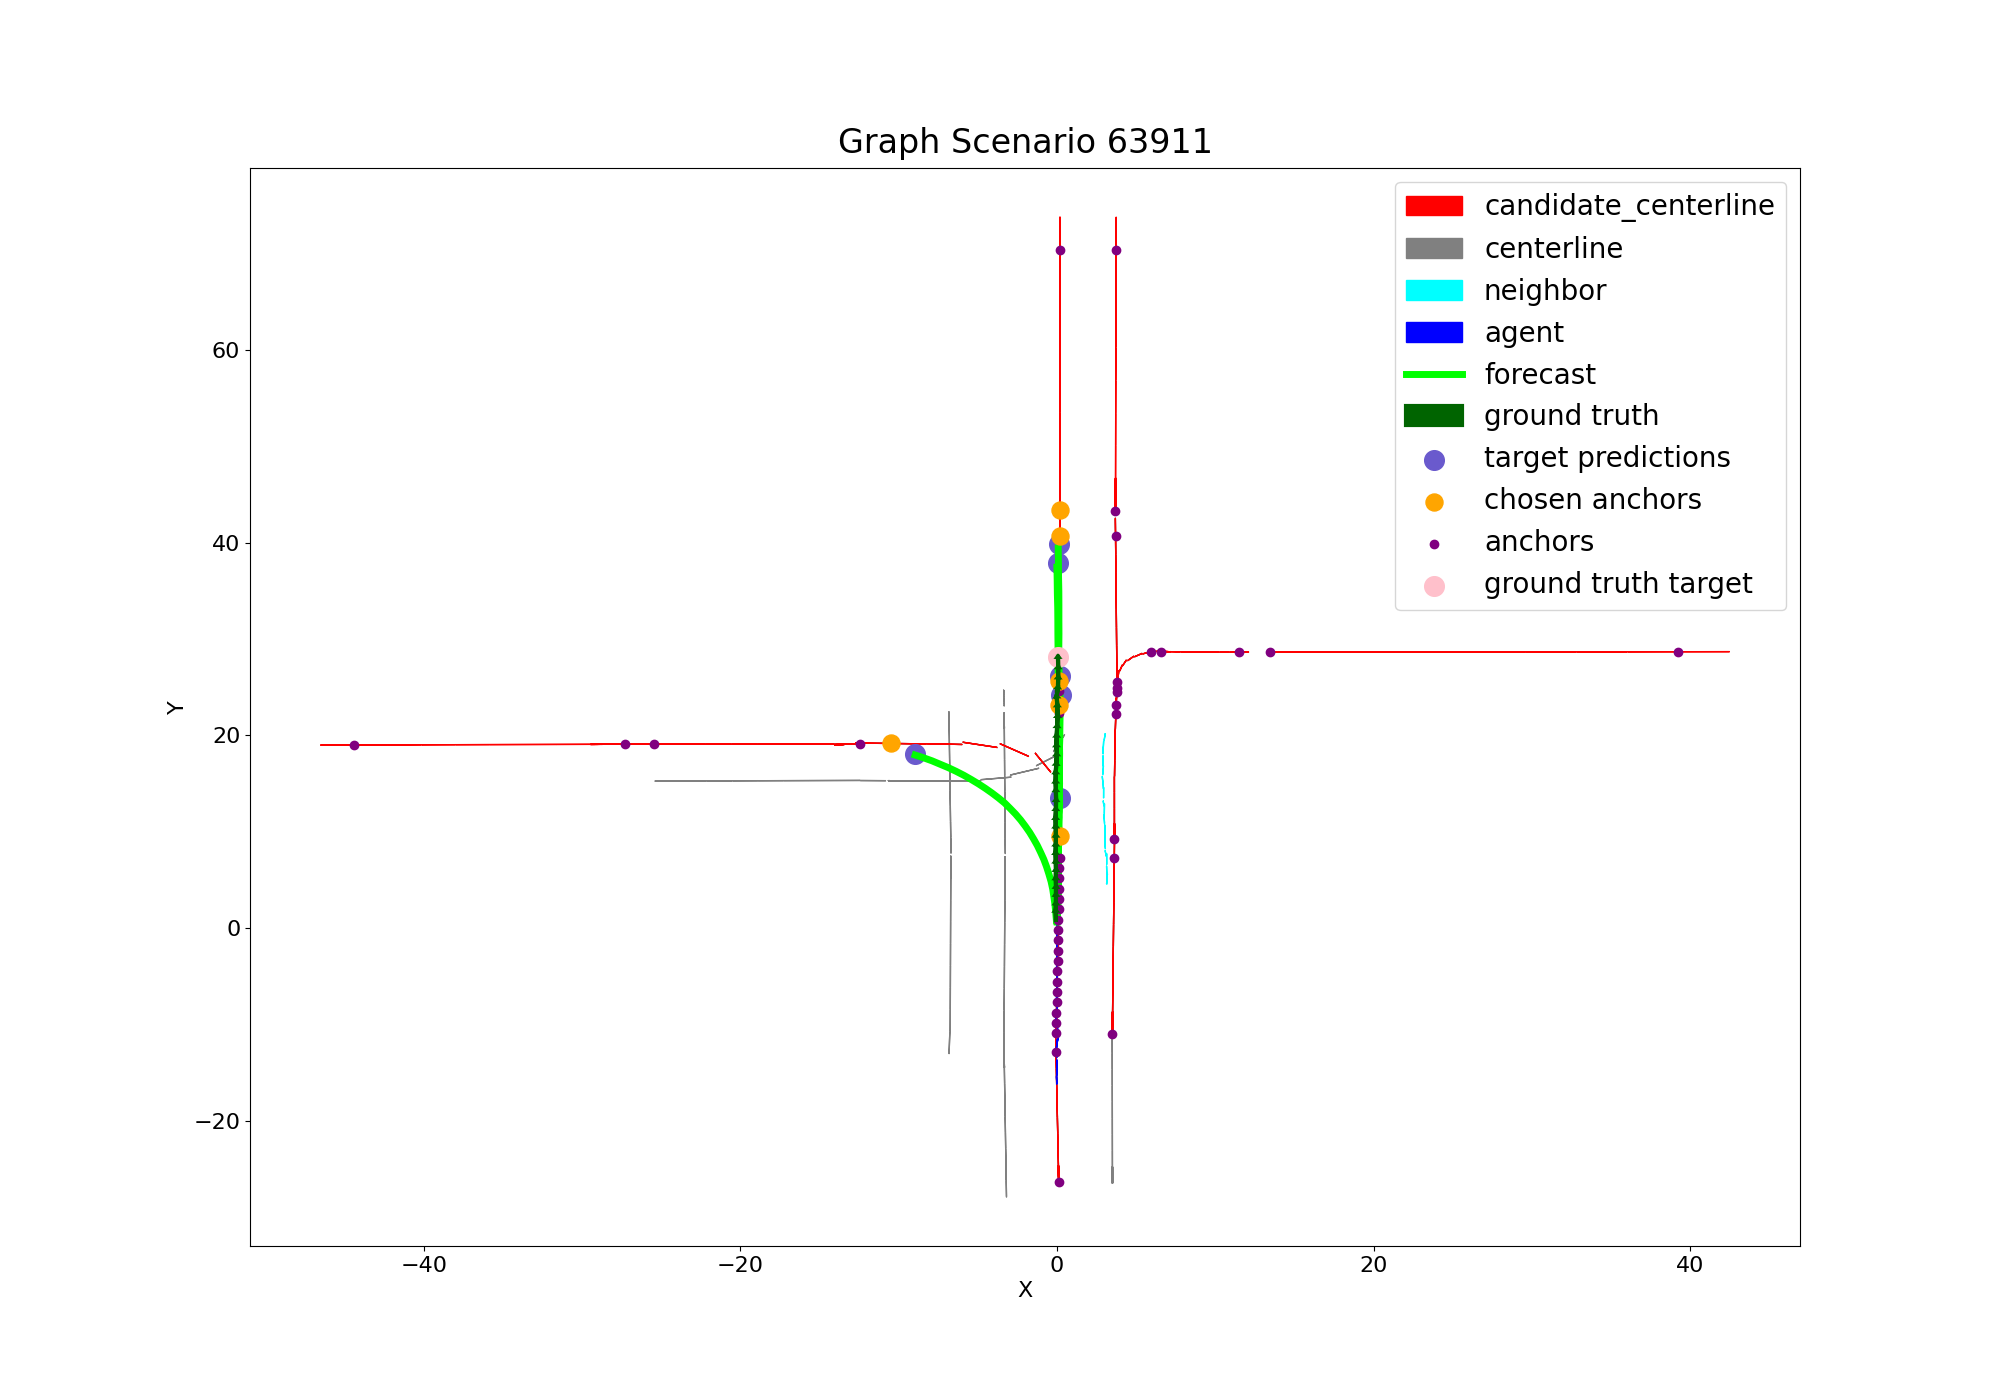
\includegraphics[width=10cm,height=7cm]{result_MIA_63911.png}
	\end{figure}
  
\end{frame}

\begin{frame}{TNT-VectorNet: Rezultati}
  \begin{figure}
		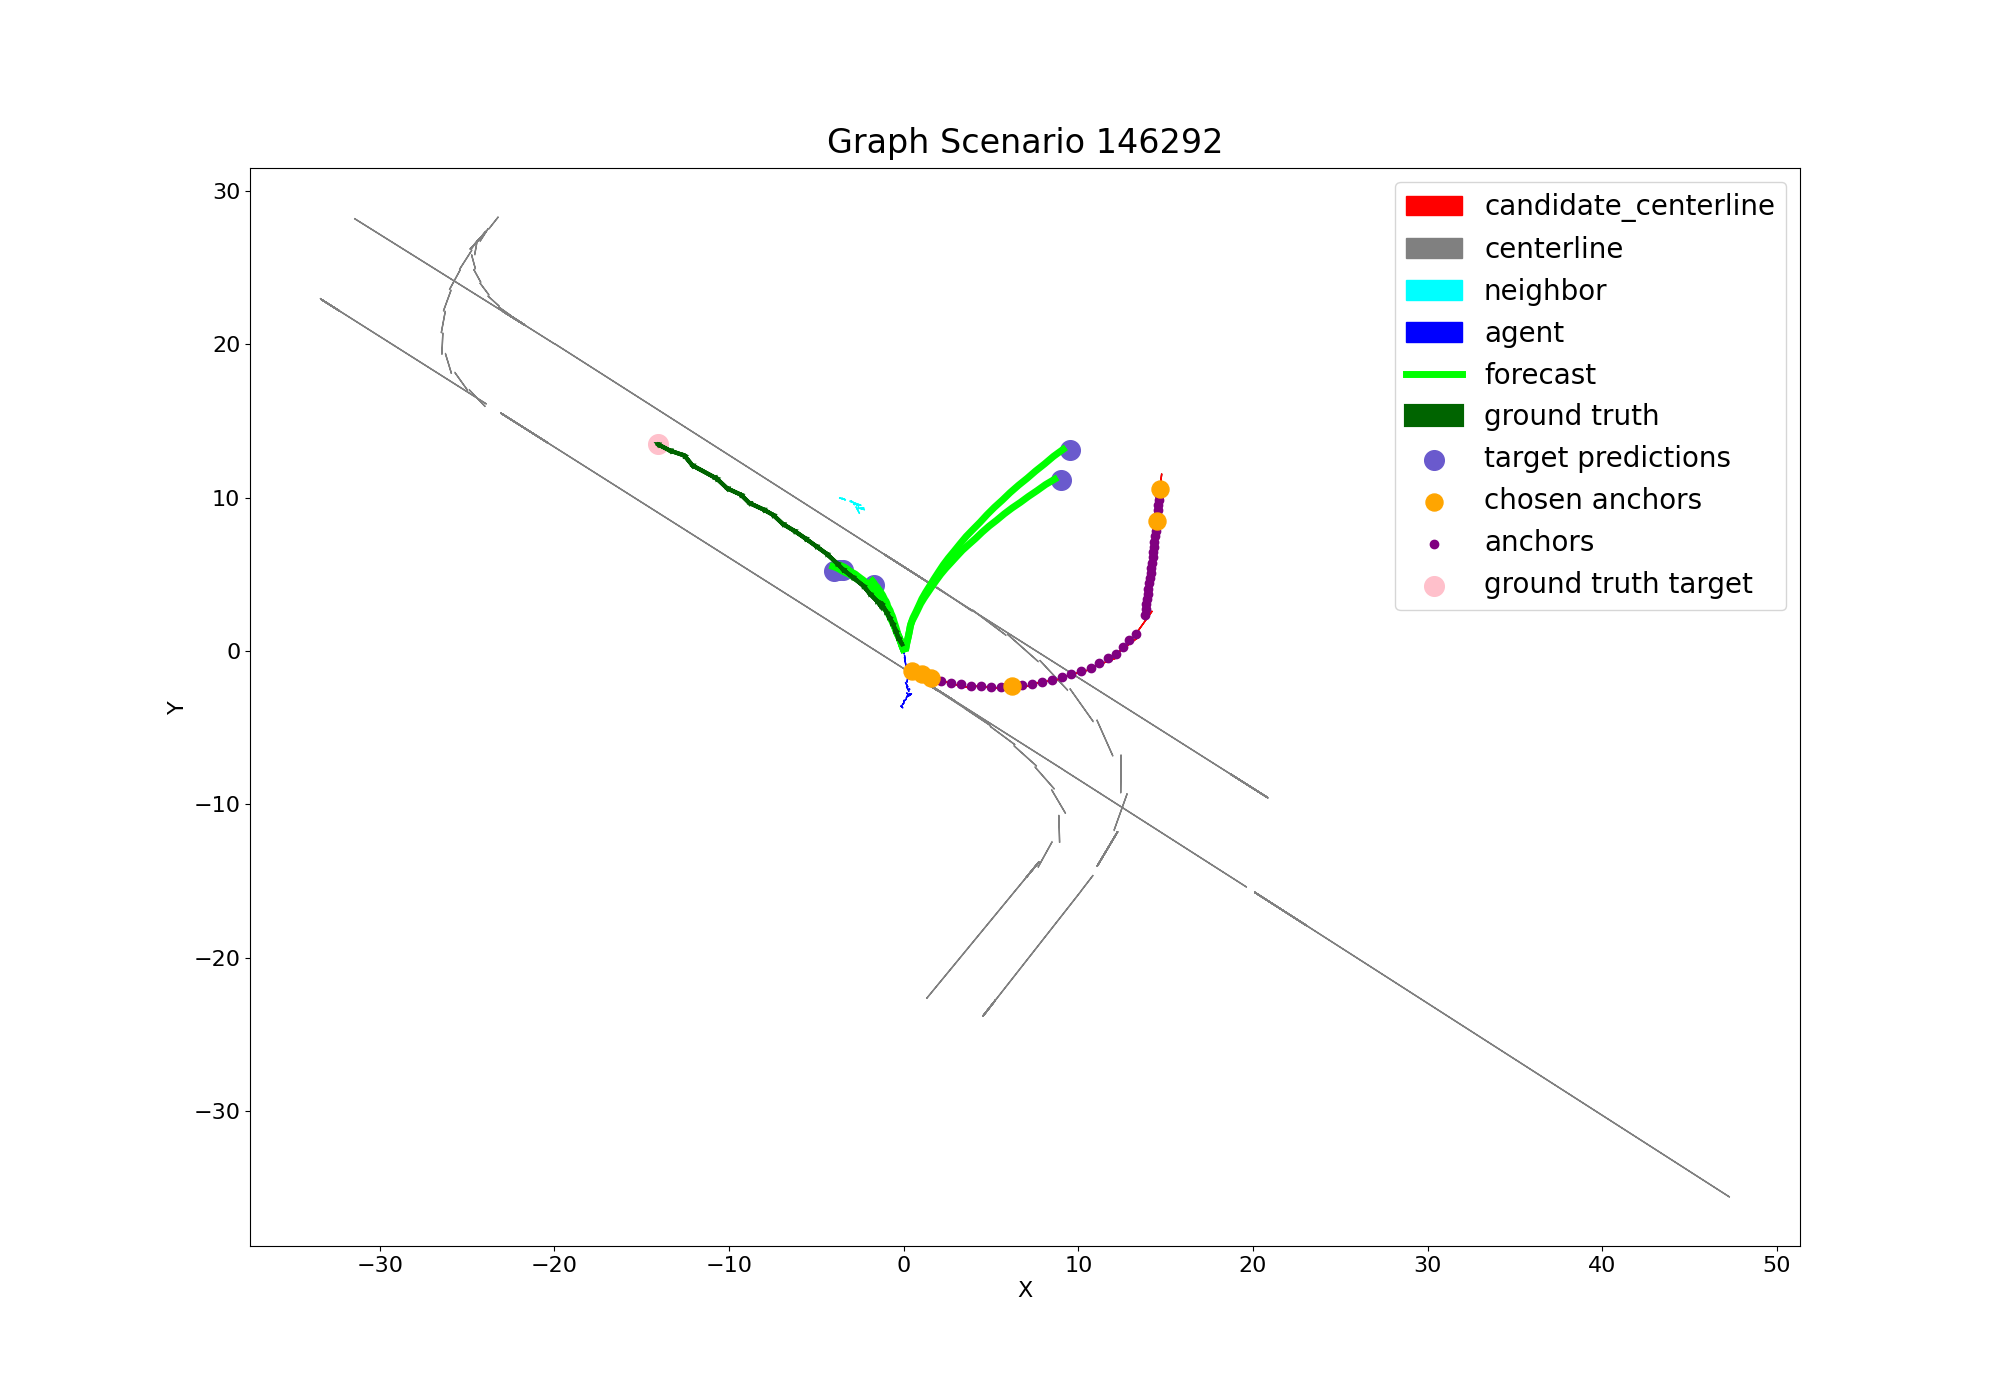
\includegraphics[width=10cm,height=7cm]{result_PIT_146292.png}
	\end{figure}
  
\end{frame}

\begin{frame}{HOME}

  \begin{itemize}
    \item Rasterizacija HD mapa (retke matrice)
    \item Estimacija toplotne mape krajnjih tačaka trajektorija agenta
    \item Osnovni gradivni element je sloj konvolutivne neuronske mreže
  \end{itemize}

  \begin{figure}
		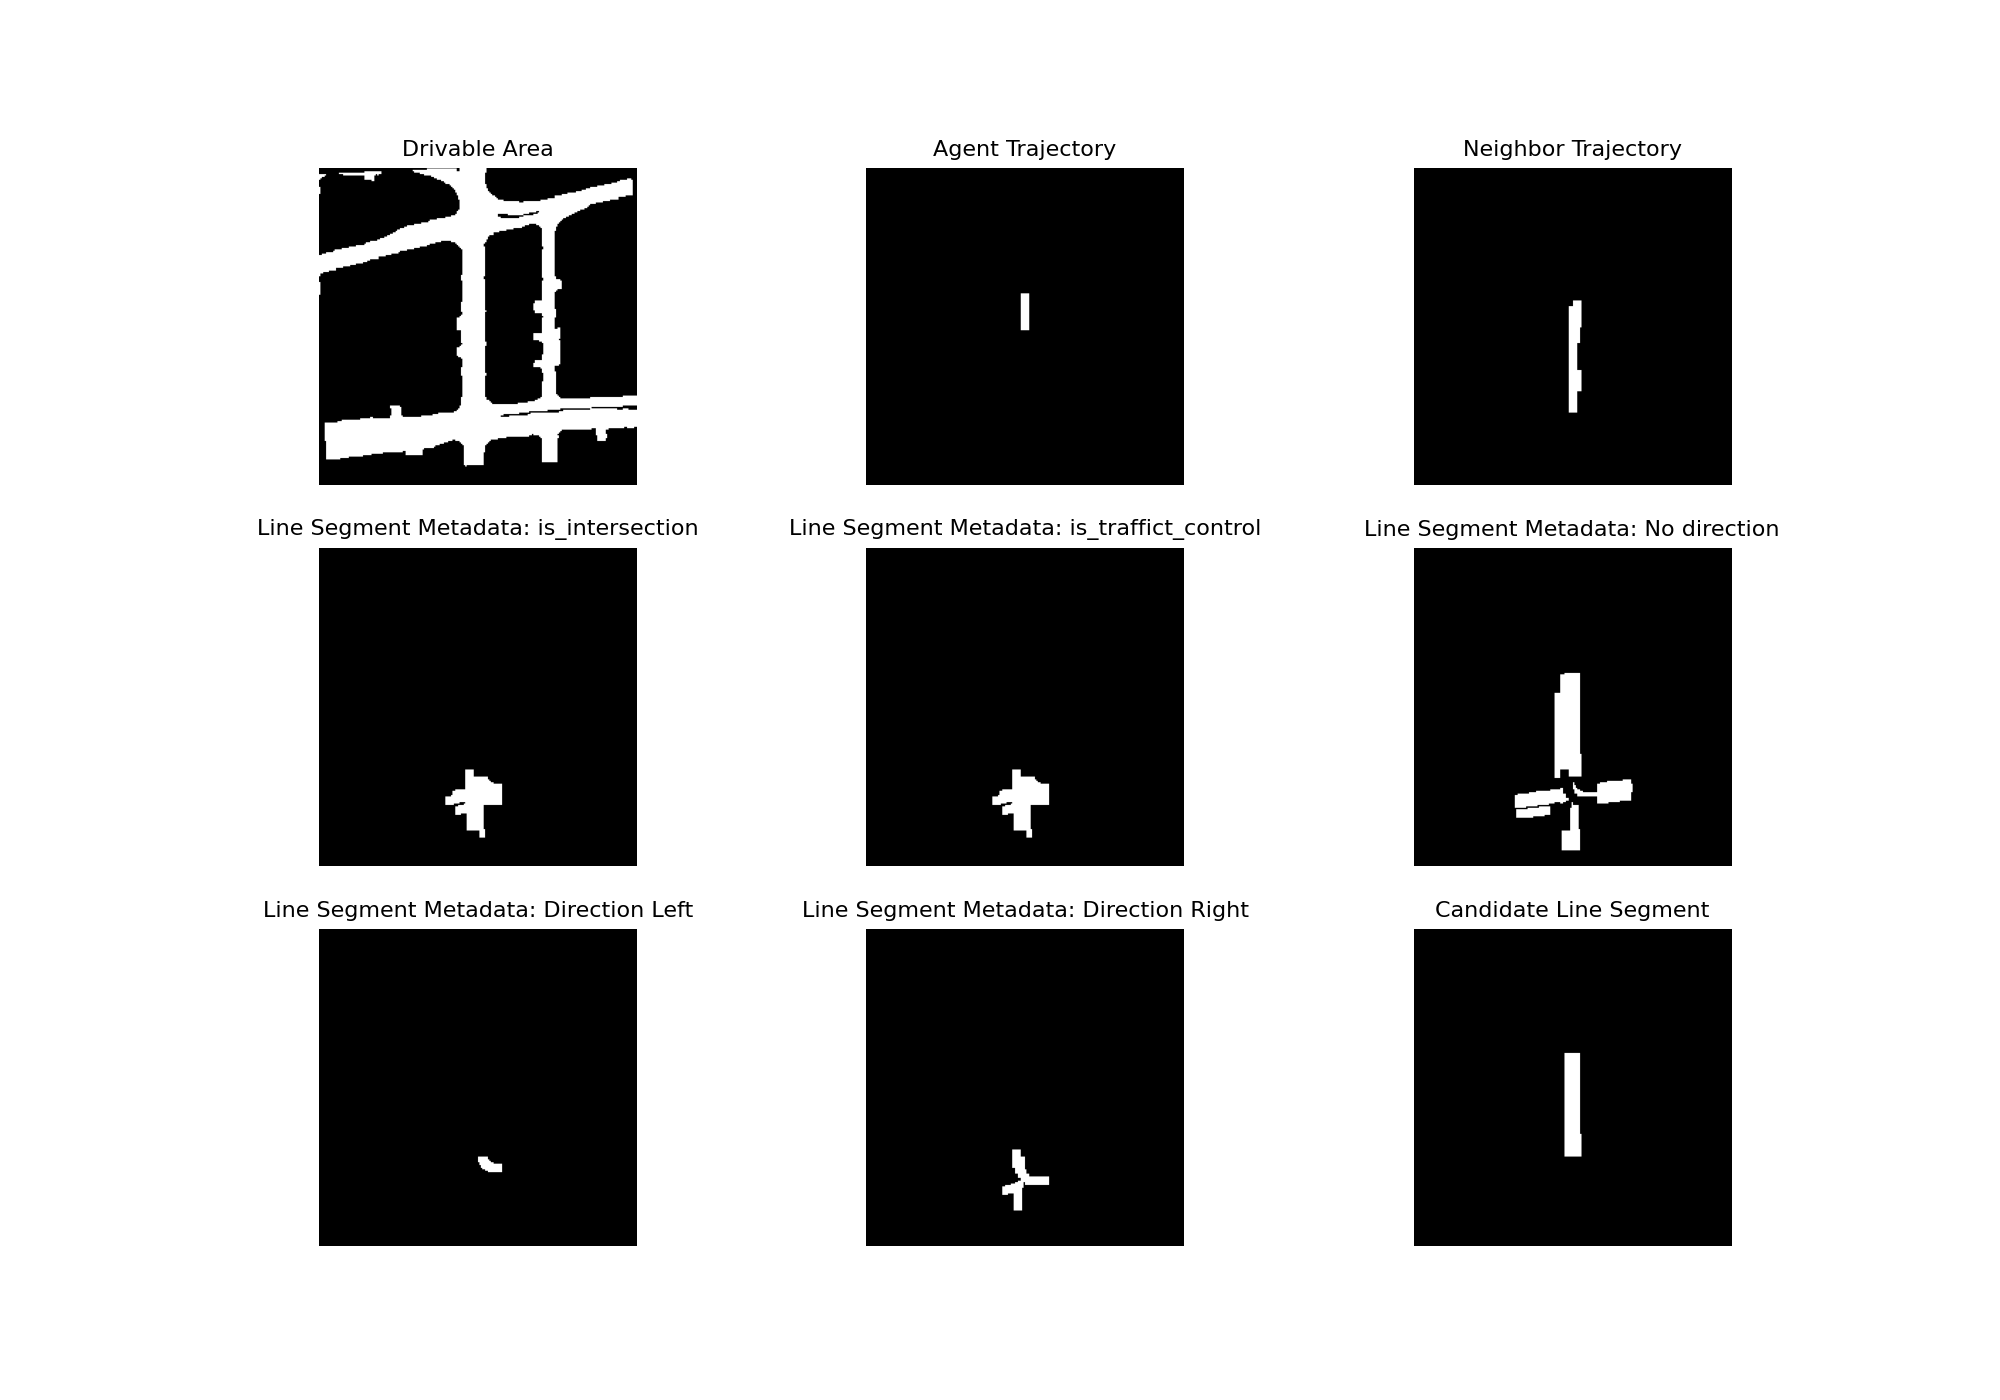
\includegraphics[width=9cm,height=6cm]{raster_MIA_24732.png}
	\end{figure}

\end{frame}

\begin{frame}{HOME: Rezultati}
  \centerline{$minADE_{6}$: $0.97$, $minFDE_{6}$: $1.71$, $MissRate^{2m}_{6}$: $0.15$}

  \begin{figure}
		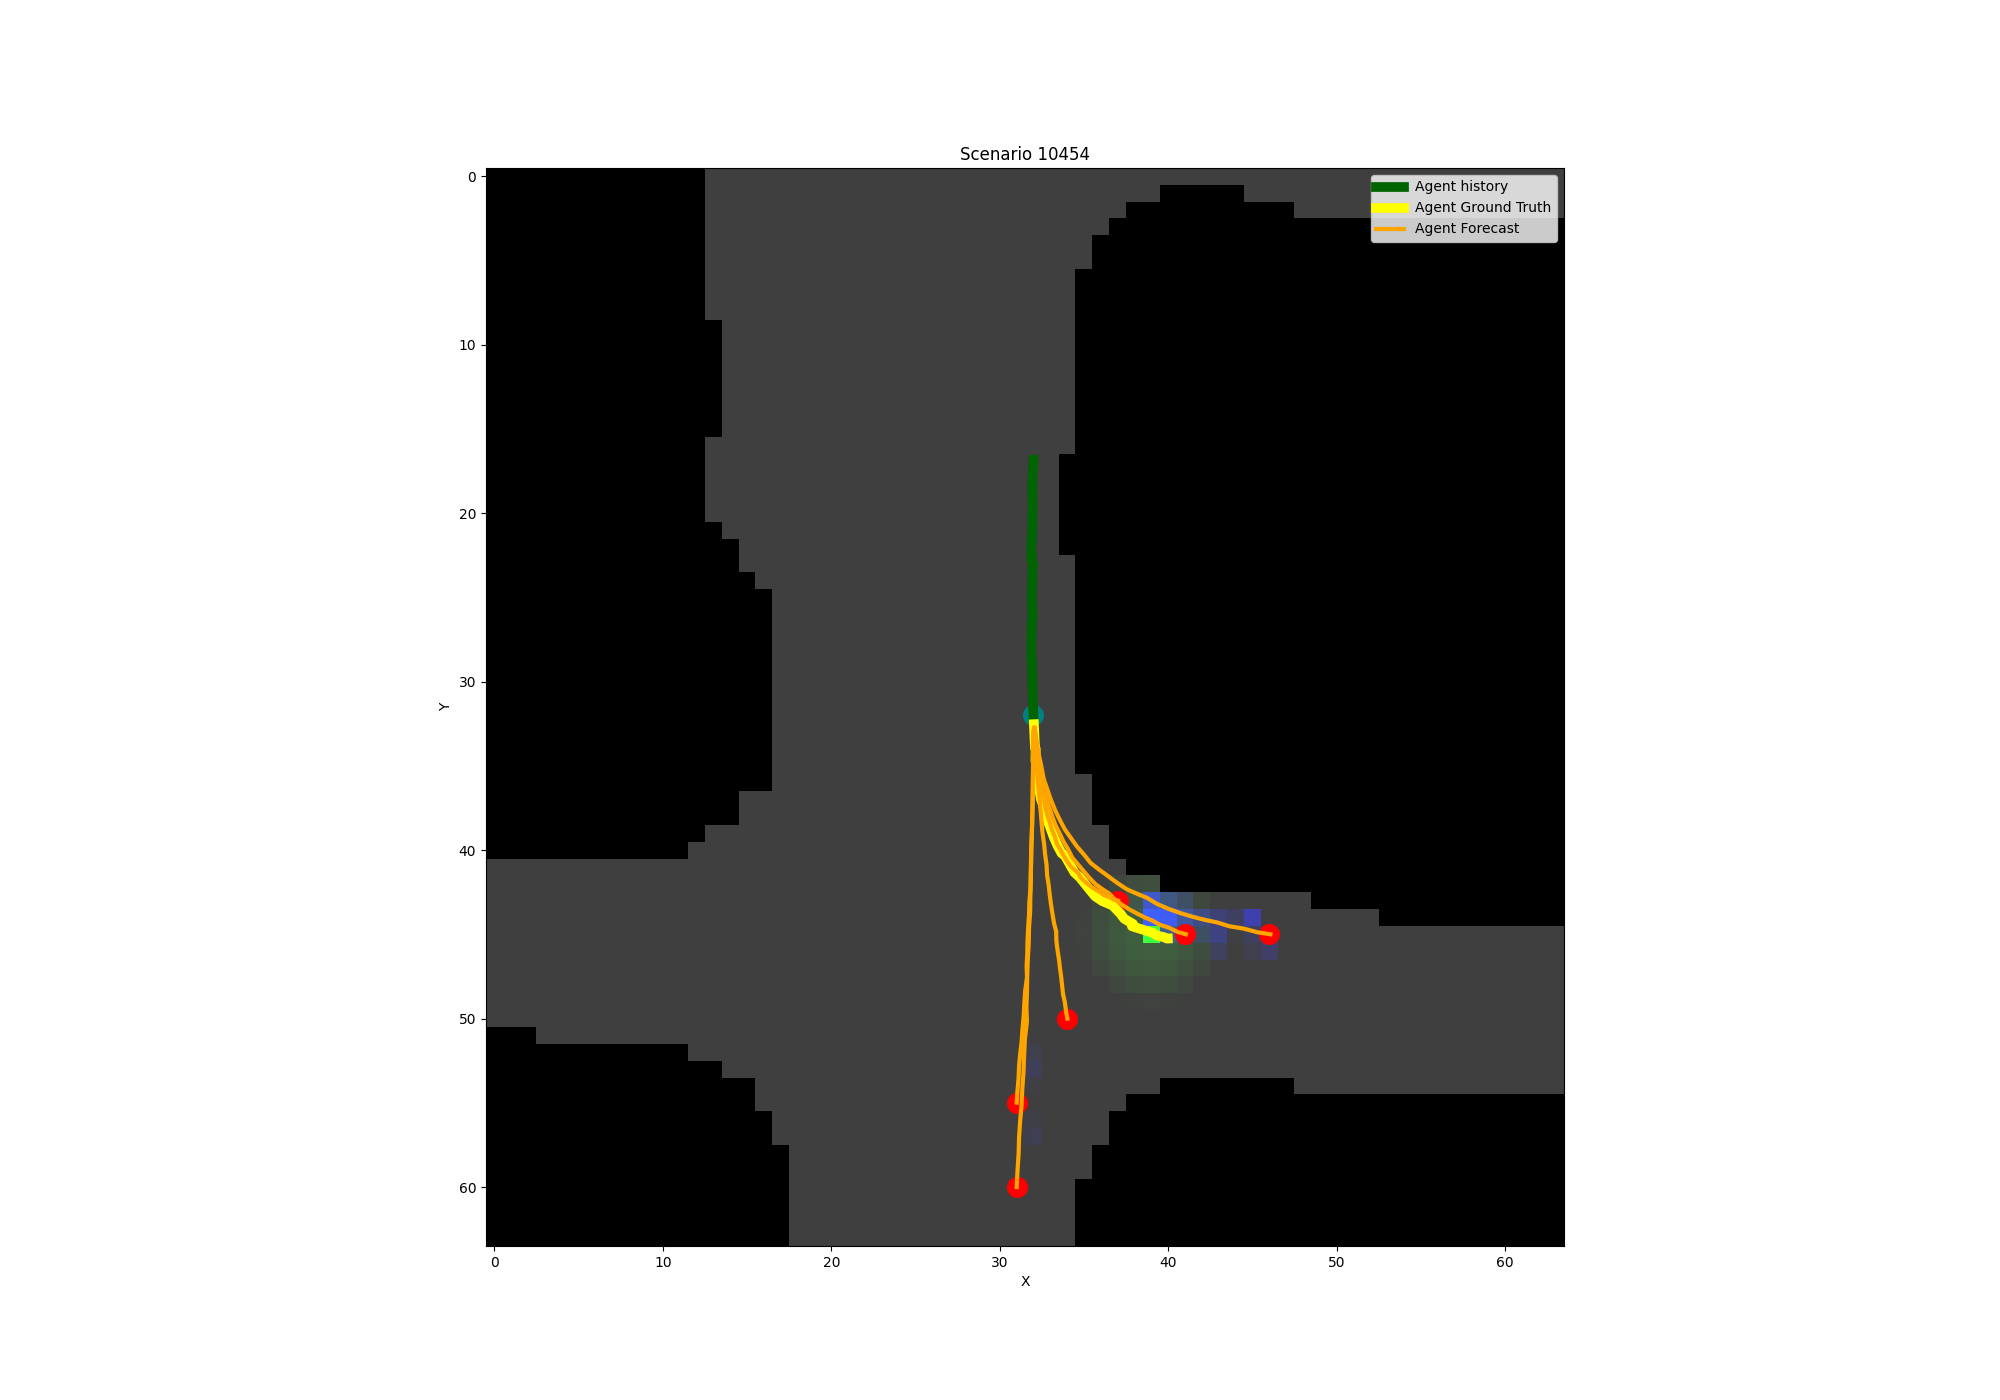
\includegraphics[width=10cm,height=7cm]{home_MIA_10454.png}
	\end{figure}
  
\end{frame}

\begin{frame}{HOME: Rezultati}
  \begin{figure}
		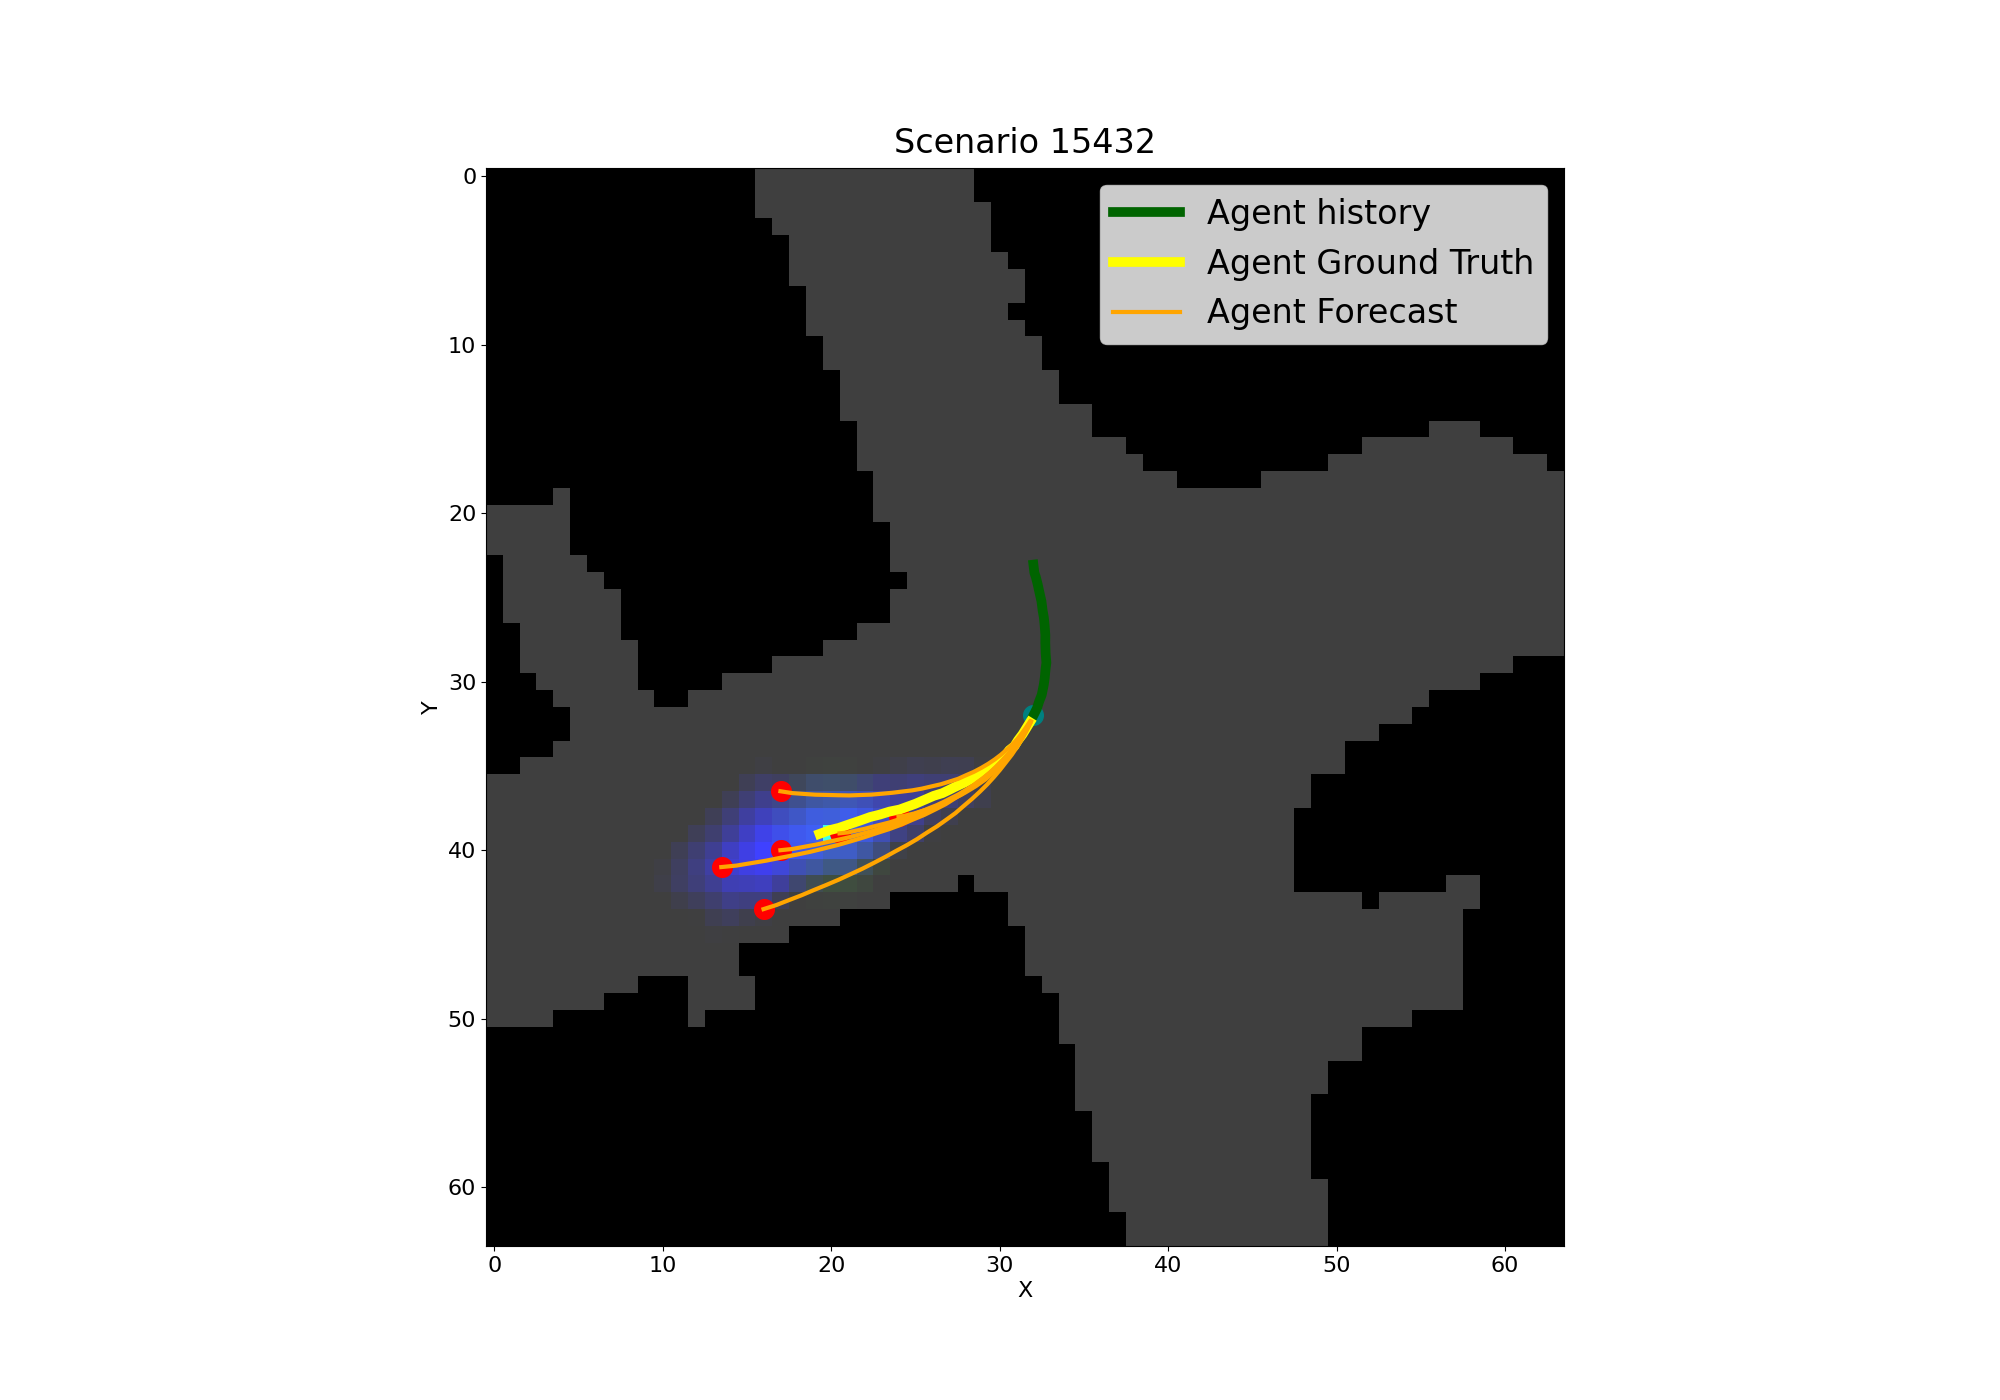
\includegraphics[width=10cm,height=7cm]{home_PIT_15432.png}
	\end{figure}
\end{frame}


\begin{frame}{HOME: Rezultati}
  \begin{figure}
		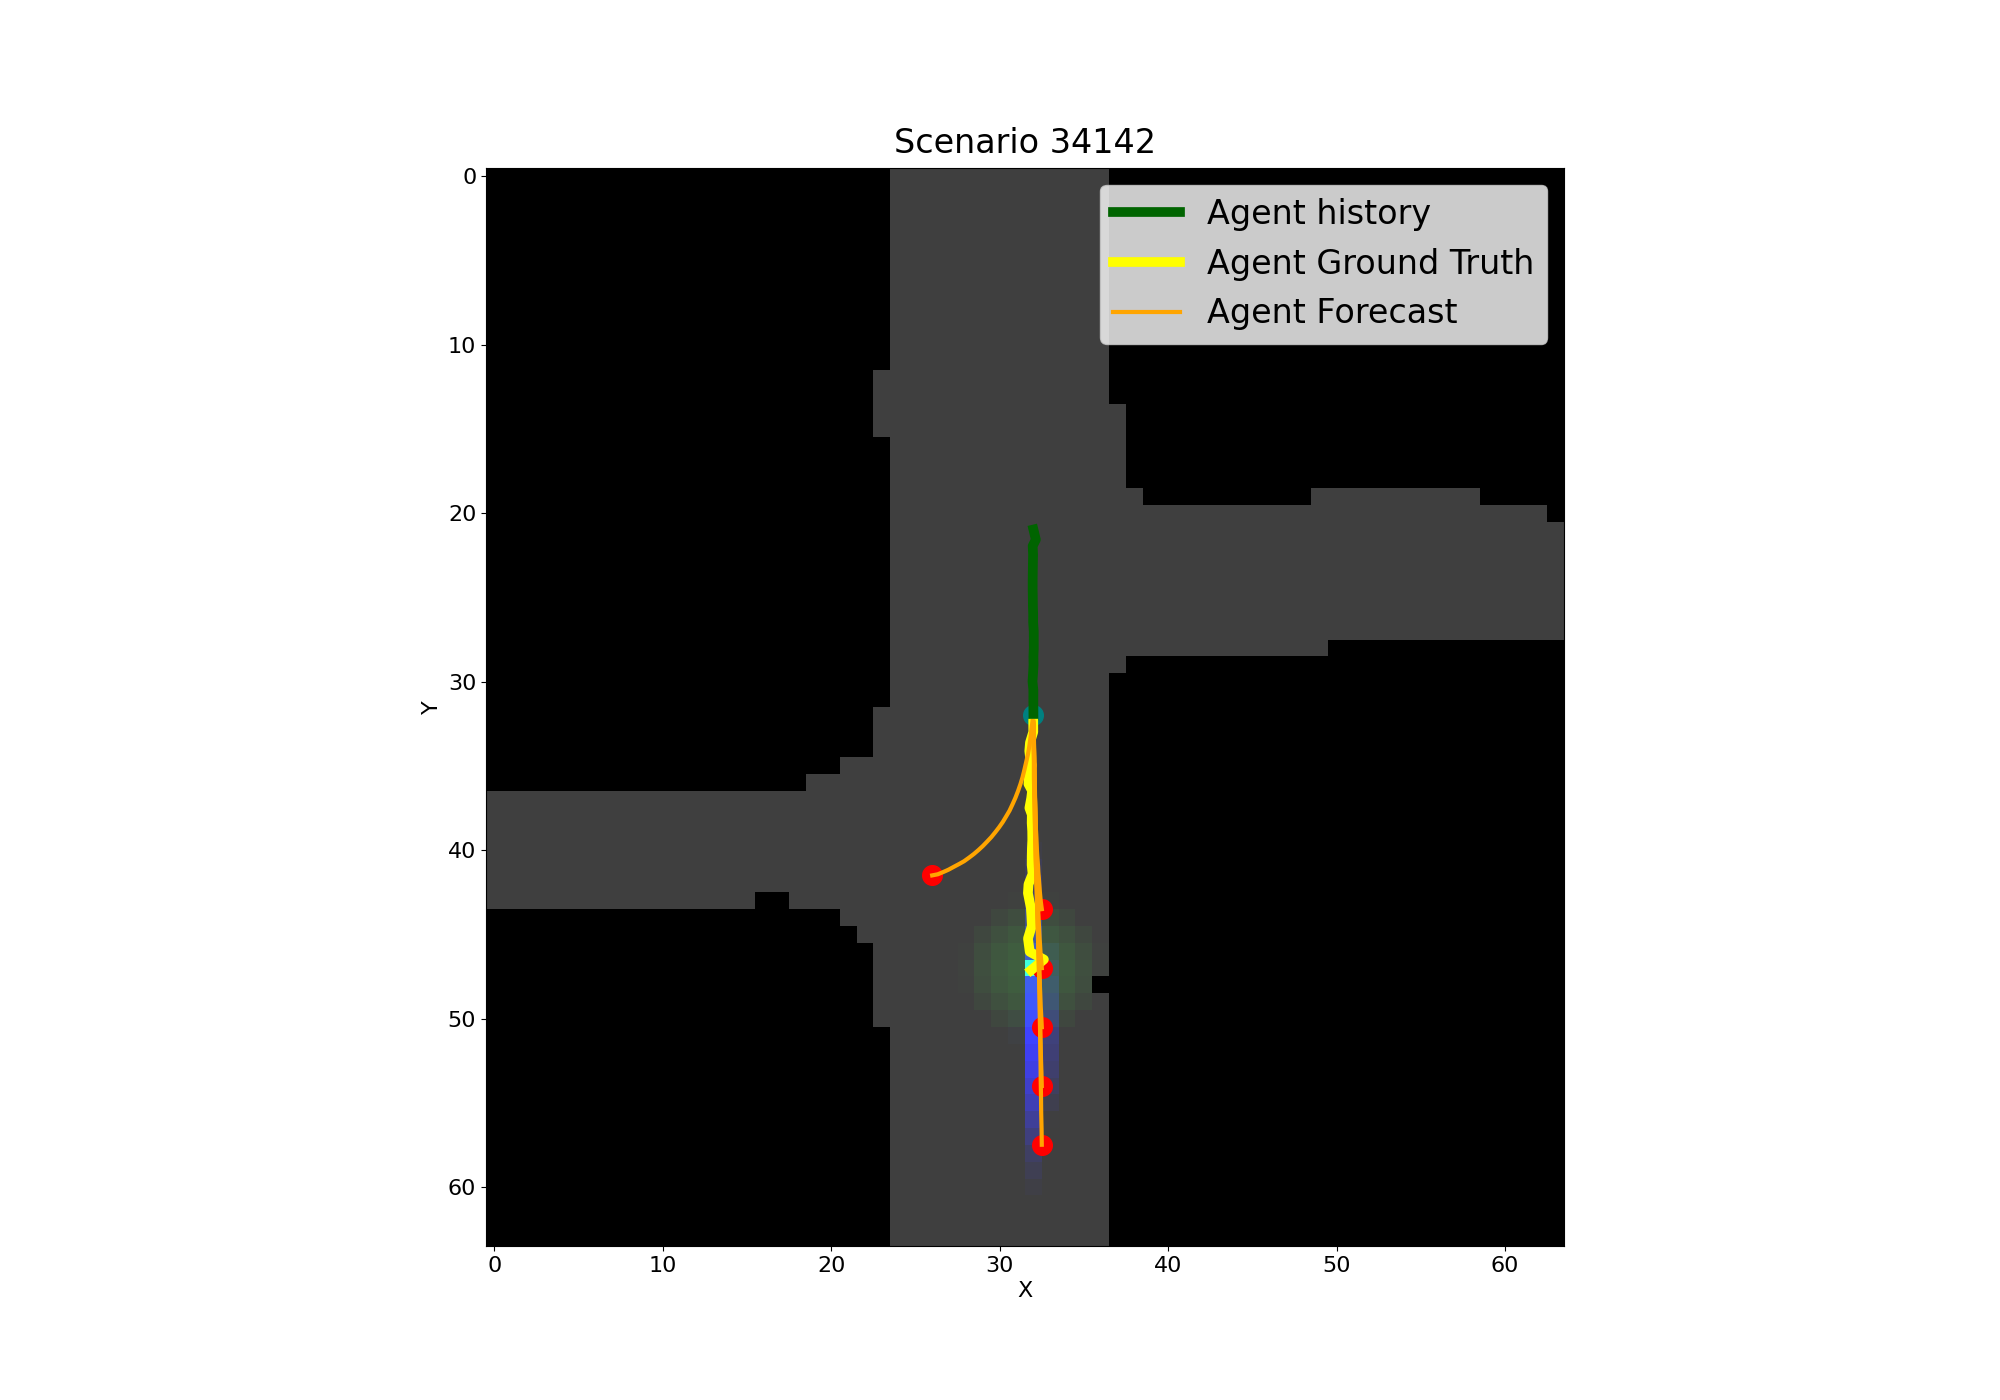
\includegraphics[width=10cm,height=7cm]{home_MIA_34142.png}
	\end{figure}
\end{frame}

\begin{frame}{HOME: Rezultati}
  \begin{figure}
		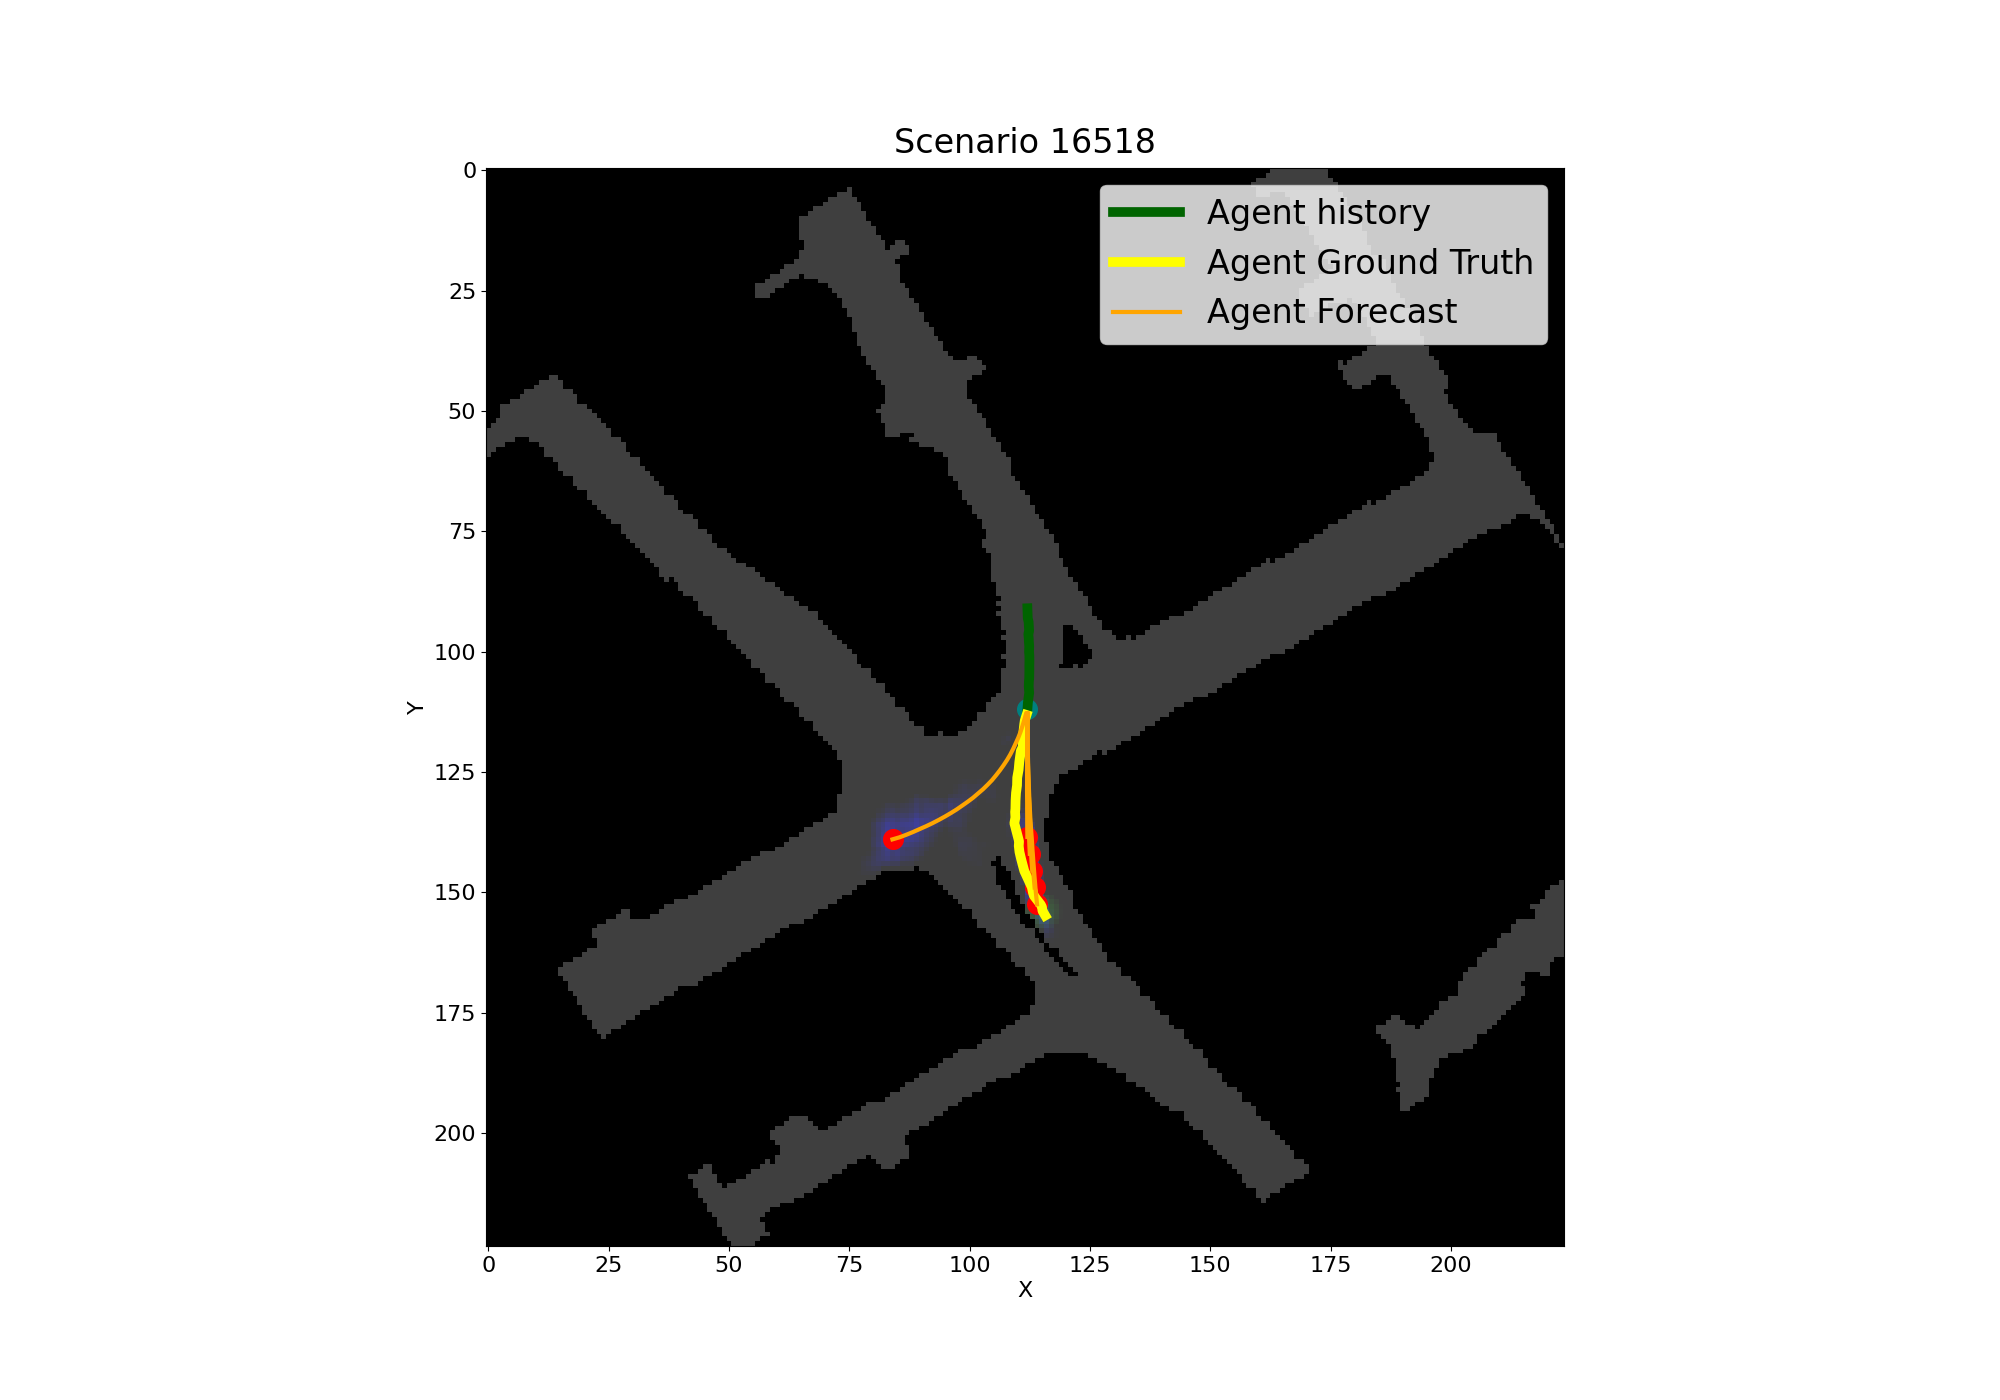
\includegraphics[width=10cm,height=7cm]{home_full_MIA_16518.png}
	\end{figure}
\end{frame}

\begin{frame}{Zaključak}

  \begin{itemize}
    \item Prednost HOME-a je što estimira uslovnu raspodelu krajnjih tačaka trajektorija, dok TNT-VectorNet koristi heuristiku (domensko znanje)
          za uzorkovanje krajnjih tačaka
    \item HOME daje bolje estimacije, ali je računski zahtevniji
    \item Postoji mogućnost kombinovanja arhitektura radi prevazilaženja postojećih ograničenja
  \end{itemize}

\end{frame}

\end{document}